\documentclass[letterpaper]{article}
\usepackage{amsmath,amssymb}
\usepackage{lmodern}
\usepackage{iftex}

\usepackage[T1]{fontenc}
\usepackage[utf8]{vietnam}
\usepackage{textcomp} % provide euro and other symbols
\usepackage{lipsum}
\usepackage{setspace}
\usepackage{adjustbox}
\usepackage{hyperref}
\usepackage{multirow}
\usepackage[table]{xcolor}
\usepackage{xcolor}
\usepackage{longtable,booktabs,array}
\usepackage{multirow}
\usepackage{calc} % for calculating minipage widths
% Correct order of tables after \paragraph or \subparagraph
\usepackage{etoolbox}

\usepackage{adjustbox}
\usepackage{graphicx}
\makeatletter
\def\maxwidth{\ifdim\Gin@nat@width>\linewidth\linewidth\else\Gin@nat@width\fi}
\def\maxheight{\ifdim\Gin@nat@height>\textheight\textheight\else\Gin@nat@height\fi}
\makeatother
% Scale images if necessary, so that they will not overflow the page
% margins by default, and it is still possible to overwrite the defaults
% using explicit options in \includegraphics[width, height, ...]{}
\setkeys{Gin}{width=\maxwidth,height=\maxheight,keepaspectratio}

\usepackage{tabularx}
% \setlength{\parskip}{1cm plus 4mm minus 3mm}
% \setlength{\parindent}{1cm}
\usepackage[top=15mm, bottom=15mm, left=30mm, right=30mm]{geometry} % page layout

% add biblatex
\usepackage[backend=bibtex,style=numeric ,natbib=true, sorting=none, maxbibnames=99]{biblatex} 
\addbibresource{ref}

% re-define section/ subsection
\usepackage{titlesec}
\providecommand{\tightlist}{%
  \setlength{\itemsep}{0pt}\setlength{\parskip}{0pt}}
\setcounter{secnumdepth}{-\maxdimen} % remove section numbering
\DeclareUnicodeCharacter{0301}{*************************************}

\titleformat{\section}
  {\large\bfseries\color{blue}}
  {\thesection}{1em}{}
\titleformat{\subsection}
  {\large\bfseries\color{blue}}
  {\thesection}{1em}{}
\titleformat{\subsubsection}
  {\normalsize\color{blue}}
  {\thesection}{1em}{}
\author{Khoa Nguyen}
\date{Oct 2023}

\begin{document}

\begin{table*}[!ht]
    \centering
    \begin{tabular}{m{6em} c  m{7em} m{5em} }
   

         \multirow{3}{3em}{
         \begin{minipage}{0.15\textwidth}
      
\includegraphics{asset/Figure/image1.png}
    \end{minipage}} & 
     & & \\  \cline{3-4}
     & \small ĐẠI HỌC QUỐC GIA TP.HCM &  \multicolumn{1}{|c|}{\multirow{2}{8em}{\small Ngày nhận hồ sơ}} &  \multicolumn{1}{|c|}{}\\
    & \small \textbf{TRƯỜNG ĐẠI HỌC CÔNG NGHỆ THÔNG TIN} & \multicolumn{1}{|c|}{} &  \multicolumn{1}{|c|}{}\\\cline{3-4}

        & & \multicolumn{2}{|c|}{\textit{\small (Do CQ quản lý ghi)}}\\ \cline{3-4}
    
    \end{tabular}
    % \caption{Caption}
    % 
\end{table*}

\begin{quote}
\centering
\textbf{\Large THUYẾT MINH}

\Large ĐỀ TÀI NGHIÊN CỨU KHOA HỌC SINH VIÊN 2024
\end{quote}


\section{A. THÔNG TIN CHUNG}

\subsection{A1. Tên đề tài}


\begin{itemize}
% \item[-]  Tên tiếng Việt (IN HOA): TĂNG CƯỜNG KHẢ NĂNG NHẬN DIỆN LỖ HỔNG TRONG HỢP ĐỒNG THÔNG MINH SỬ DỤNG MÔ HÌNH NGÔN NGỮ LỚN VÀ NHẬN DIỆN NÚT NHẠY CẢM
% \item[-]  Tên tiếng Anh (IN HOA): ENHANCING SMART CONTRACT VULNERABILITY DETECTION USING LARGE LANGUAGE MODEL AND SENSITIVE NODE IDENTIFICATION
\item[-]  Tên tiếng Việt (IN HOA): MỘT HƯỚNG TIẾP CẬN TINH CHỈNH MÔ HÌNH NGÔN NGỮ LỚN VÀ TỐI ƯU CHUỖI TỪ ĐỒ THỊ CÂY CÚ PHÁP TRỪU TƯỢNG TRONG PHÁT HIỆN LỖ HỔNG HỢP ĐỒNG THÔNG MINH 
\item[-]  Tên tiếng Anh (IN HOA): A NOVEL APPROACH TO FINE-TUNING LARGE LANGUAGE MODELS AND OPTIMIZING ABSTRACT SYNTAX TREE SEQUENCES FOR SMART CONTRACT VULNERABILITY DETECTION
\end{itemize}


\subsection{A2. Thời gian thực hiện}

6 tháng (kể từ khi được duyệt).

\subsection{A3. Tổng kinh phí}

\noindent Tổng kinh phí: 6 triệu đồng, gồm:

\begin{itemize}
\item
  Kinh phí từ Trường Đại học Công nghệ Thông tin: 6 triệu
  đồng
\end{itemize}


\subsection{A4. Chủ nhiệm}
\begin{spacing}{1.5}

\indent \indent Họ và tên: Nguyễn Hải Phong \par

Ngày, tháng, năm sinh: 14/05/2004  \hspace{2cm} Giới tính (Nam/Nữ): Nam\par

Số CCCD: 079204006385 \hspace{3cm}; Ngày cấp: 26/09/2018 \hspace{3cm}; Nơi cấp: Cục Cảnh Sát Quản Lý Hành Chính Và Trật Tự Xã Hội

Mã số sinh viên:  22521088

Số điện thoại liên lạc: 0903792388

Khoa:  Mạng Máy tính và Truyền thông

Số tài khoản: 9704186930001196015 \hspace{4cm} Ngân hàng: BIDV Tân Bình
\end{spacing}

\subsection{A5. Thành viên đề tài (kể cả CNĐT)}


\begin{longtable}[c]{@{}
  >{\raggedright\arraybackslash}p{(\columnwidth - 6\tabcolsep) * \real{0.0553}}
  >{\raggedright\arraybackslash}p{(\columnwidth - 6\tabcolsep) * \real{0.3235}}
  >{\raggedright\arraybackslash}p{(\columnwidth - 6\tabcolsep) * \real{0.3637}}
  >{\raggedright\arraybackslash}p{(\columnwidth - 6\tabcolsep) * \real{0.2575}}@{}}
\toprule()
\begin{minipage}[b]{\linewidth}\raggedright
\textbf{TT}
\end{minipage} & \begin{minipage}[b]{\linewidth}\raggedright
\textbf{Họ tên}
\end{minipage} & \begin{minipage}[b]{\linewidth}\raggedright
\textbf{MSSV}
\end{minipage} & \begin{minipage}[b]{\linewidth}\raggedright
\textbf{Khoa}
\end{minipage} \\
\midrule()
\endhead
1 & Nguyễn Hải Phong & 22521088 & Mạng Máy tính và Truyền thông \\
2 & Nguyễn Chí Thành & 22521350 & Mạng Máy tính và Truyền thông \\
\bottomrule()
\end{longtable}




\section{B. MÔ TẢ NGHIÊN CỨU}



\subsection{B1. Giới thiệu về đề tài}

\indent \indent Công nghệ Blockchain đang chứng kiến sự phát triển liên tục và thu hút sự quan tâm đáng kể từ cả giới học thuật và thương mại. Hệ thống blockchain sở hữu những đặc tính mới như tính phân tán, tính bất biến và tính minh bạch. Những đặc điểm này được ứng dụng rộng rãi trong nhiều lĩnh vực của công nghệ blockchain, không chỉ giới hạn trong tiền ảo mà còn được triển khai trong lĩnh vực chăm sóc sức khỏe, tài chính kỹ thuật số và chuỗi cung ứng thực phẩm, v.v. Ethereum là một trong những nền tảng blockchain tiên phong. Một khối lượng lớn hợp đồng thông minh (smart contract) đã được triển khai trên nền tảng này, kiểm soát một lượng lớn tiền tệ và giao dịch. Hiện nay, các hợp đồng thông minh ngày càng trở nên phức tạp, với nhiều tính năng và tương tác đa dạng trong hệ sinh thái blockchain. Điều này dẫn đến việc xuất hiện nhiều lỗ hổng bảo mật khó phát hiện và dễ bị khai thác. Một ví dụ điển hình là vụ tấn công KyberSwap, một nền tảng blockchain của Việt Nam vào năm 2023, khi tin tặc đã khai thác lỗ hổng reentrancy trong một hợp đồng thông minh KS2-RT, dẫn đến thất thoát với ước tính 47 triệu đô la bị đánh cắp. Kẻ tấn công liên tục sử dụng các kỹ thuật tiên tiến để vượt qua các cơ chế bảo mật và khai thác các điểm yếu. Những kỹ thuật này bao gồm làm rối mã (obfuscation), chèn mã (code injection),...\cite{zhang2023bian}. Những sự cố này không chỉ gây ra tổn thất kinh tế lớn mà còn đe dọa tính an toàn của các hệ thống blockchain. Chính những điều trên đã đặt nhu cầu lớn đối với việc phải có những phương thức, phương pháp để đảm bảo được tính an toàn và tin cậy của các hợp đồng thông minh trong lĩnh vực blockchain.

\indent Trước thực trạng ấy, trong những năm gần đây đã có nhiều phương pháp được đề xuất để khắc phục vấn đề này. Một trong những phương pháp phổ biến là phương pháp áp dụng mô hình mạng nơ-ron đồ thị (Graph Neural Network - GNN) trong quá trình phân tích và nhận diện lỗ hổng tiềm tàng trong hợp đồng thông minh. Một số nghiên cứu về phương pháp này có thể nhắc đến như công trình nghiên cứu \cite{liu2021combining} áp dụng mô hình mạng nơ-ron đồ thị cùng kiến thức chuyên môn trong việc nhận dạng lỗ hổng hợp đồng thông minh, cụ thể hơn, công trình nghiên cứu đã cho ra kết quả vượt trội về nhiều mặt so với các công cụ phân tích tĩnh hợp đồng thông minh cũng như các mô hình máy học dùng để nhận diện lỗ hổng hợp đồng thông minh như LSTM, Vanillia-RNN, ... Đồng thời cũng có thể kể đến công trình sử dụng mô hình nhận diện lỗ hổng hợp đồng thông minh ở mức sâu hơn khi chỉ định được vị trí dòng code đang tồn tại lỗ hổng trên \cite{sendner2023g}.

\indent Tuy nhiên, việc phát triển các mô hình đồ thị như mạng nơ-ron đồ thị như GNN hiệu quả để phát hiện lỗ hổng trong hợp đồng thông minh đòi hỏi kiến thức chuyên môn sâu rộng và kỹ năng xử lý đặc trưng phức tạp. Hiệu quả của các mô hình này phụ thuộc đáng kể vào chất lượng và tính đầy đủ của biểu diễn đồ thị, vốn phải phản ánh chính xác các tương tác và logic bên trong hợp đồng. Biểu diễn không đầy đủ hoặc thiếu chính xác có thể dẫn đến việc bỏ sót các lỗ hổng quan trọng, làm giảm khả năng phát hiện và phân tích của mô hình.

\indent Trong bối cảnh đó, sự phát triển của các mô hình ngôn ngữ lớn (Large Language Models - LLMs) đã mang lại một giải pháp thay thế đáng chú ý, với khả năng xử lý ngữ cảnh và phân tích chuỗi văn bản dài vượt trội. Do đó, việc lựa chọn mô hình phù hợp để phát hiện lỗ hổng trong hợp đồng thông minh cần được cân nhắc kỹ lưỡng. Các LLM mã nguồn mở, được tối ưu hóa cho học chuyển giao (transfer learning), được ưu tiên sử dụng nhằm cân bằng giữa hiệu quả và tài nguyên. Tuy nhiên, hạn chế của các LLM này là giới hạn số lượng token, chẳng hạn như BERT với tối đa chỉ 512 tokens, rất hạn chế so với độ dài token trung bình của các hợp đồng thông minh sau khi xử lý hiện nay. Vì vậy, các mô hình được lựa chọn cần đảm bảo tính gọn nhẹ, sử dụng số lượng tham số hợp lý để vừa duy trì hiệu suất cao vừa giảm thiểu yêu cầu tài nguyên, từ đó nâng cao tính ứng dụng thực tiễn.

\begin{figure}[!hbt]
    \centering
    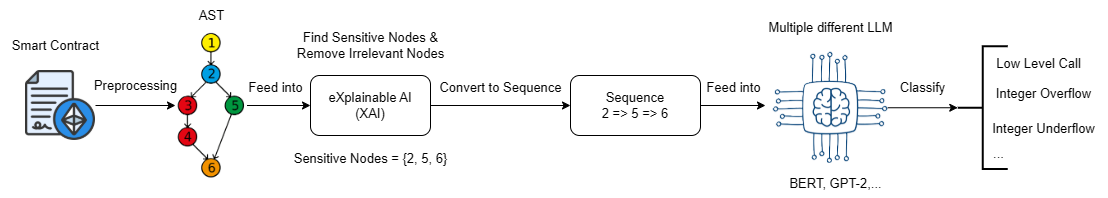
\includegraphics[width=1\linewidth]{Figures/Tong_Quan_Mo_Hinh_NCKH.png}
    \caption{Tổng quan về mô hình đề xuất.}
    \label{fig:enter-label}
\end{figure}

% \indent Để tối ưu hóa hơn nữa, nghiên cứu sẽ tiến hành giảm chiều dữ liệu, sao cho vẫn giữ được ngữ nghĩa của chuỗi nhưng không làm giảm hiệu quả trong việc phân loại lỗ hổng hợp đồng thông minh. Điều này giúp duy trì tính chính xác cao và đảm bảo khả năng xử lý hiệu quả các chuỗi văn bản phức tạp.

\subsection{B2. Mục tiêu, nội dung, kế hoạch nghiên cứu}
\subsection{B2.1 Mục tiêu}

\begin{itemize}
    \item Đề xuất một cách tiếp cận phát hiện và phân loại lỗ hổng hợp đồng thông minh bằng cách chuyển đồ thị cây cú pháp trừu tượng (Abstract Syntax Tree - AST) thành chuỗi có ngữ nghĩa (sequence). Chuỗi này được xử lý bởi các mô hình ngôn ngữ lớn như BERT, CodeBERT, GraphCodeBERT, GPT-2 để phân tích và nhận diện lỗ hổng với độ chính xác cao.

    \item Sử dụng phương pháp trí tuệ nhân tạo khả diễn giải (eXplainable AI - XAI), cụ thể là kỹ thuật SHapley Additive exPlanations (SHAP) \cite{lundberg2017unified_shap}, để tìm và tập trung vào những nút nhạy cảm trong đồ thị, loại bỏ các nút không liên quan. Sau đó, thuật toán duyệt theo chiều sâu (DFS) được áp dụng để chuyển đồ thị thành chuỗi mà vẫn giữ nguyên luồng thực thi của loại tấn công, giúp giảm khối lượng xử lý của LLM và cải thiện hiệu suất.

    \item Tập dữ liệu SoliAudit (17,980 mẫu từ Ethereum và CTF) \cite{liao2019soliaudit} được sử dụng để huấn luyện mô hình. Phương pháp kết hợp các đặc điểm của đồ thị con và XAI giúp mô hình không chỉ phát hiện chính xác mà còn mở rộng khả năng nhận diện nhiều loại lỗ hổng khác nhau.
\end{itemize}


\subsection{B2.2 Nội dung và phương pháp nghiên cứu}
\subsubsection{Nội dung 1: Nghiên cứu về kiến trúc, cách thức hoạt động và tìm hiểu về các lỗ hổng phổ biến trong hợp đồng thông minh.}

\paragraph{Mục tiêu:}
\begin{itemize}
    \item Nắm được nguyên tắc hoạt động và huấn luyện mô hình được đề xuất trên.
    \item Tìm hiểu về các lỗ hổng phổ biến trong hợp đồng thông minh.
\end{itemize}

\paragraph{Phương pháp thực hiện:}

\begin{itemize}
    \item Khảo sát, triển khai và huấn luyện từng mô hình trên.
    \item Triển khai thu thập và chuẩn bị bộ dữ liệu các lỗ hổng phổ biến trong hợp đồng thông minh để huấn luyện và thử nghiệm khả năng tìm điểm nhạy cảm và phân loại của các mô hình LLM.
\end{itemize}

\paragraph{Kết quả dự kiến:}

\begin{itemize}
    \item Báo cáo về khả năng phân loại các lỗ hổng phổ biến của các mô hình LLM.
    \item Báo cáo về ưu và nhược điểm của các mô hình trước các cuộc tấn công.
\end{itemize}

\subsubsection{Nội dung 2: Nghiên cứu về phương pháp tiền xử lý đồ thị chuyển từ dạng đồ thị sang dạng sequence kết hợp với XAI}

\paragraph{Mục tiêu:}
\begin{itemize}
    \item Hiểu được phương pháp chuyển từ hợp đồng thông minh thành dạng đồ thị, cách hoạt động của XAI.
    \item Xây dựng được thuật toán tiền xử lý hợp đồng thông minh để đưa vào XAI.
    \item Xây dựng phương pháp chuyển từ đồ thị sang dạng chuỗi.
\end{itemize}

\paragraph{Phương pháp thực hiện:}
\begin{itemize}
    \item Xây dựng thuật toán chuyển từ hợp đồng thông minh thành dạng đồ thị AST.
    \item Xây dựng XAI để tìm ra những nút nhạy cảm.
    \item Dựa trên những nút nhạy cảm đó, xây dựng phương pháp để ứng dụng DFS vào duyệt đồ thị.
    \item Từ những đồ thị con đó, tạo ra được các sequence để đưa vào mô hình.
\end{itemize}

\paragraph{Kết quả dự kiến:}
\begin{itemize}
    \item Báo cáo phương pháp tiền xử lý để đưa ra AST.
    \item Báo cáo về khả năng phân tích và đưa ra những nút nhạy cảm của thuật toán.
    \item Báo cáo về ưu và nhược điểm của phương pháp này so với các phương pháp chuyển đổi khác trong các nghiên cứu.
\end{itemize}

\subsubsection{Nội dung 3: Nghiên cứu về phương pháp tiền xử lý dữ liệu (tokenizer) chuyển các chuỗi có ngữ nghĩa từ các dữ liệu dạng đồ thị như AST để LLMs phân loại nhãn về lỗ hổng phổ biến trong hợp đồng thông minh}

\paragraph{Mục tiêu:}

\begin{itemize}
    \item Nắm được lí thuyết và phương pháp tiền xử lý (tokenizer) dữ liệu dạng chuỗi (sequence) để chuẩn bị cho việc huấn luyện mô hình ngôn ngữ lớn.
    \item Nắm được kiến thức về mô hình ngôn ngữ lớn, xây dựng và hiểu được cơ chế hoạt động cũng như hiểu được ưu và nhược điểm của mô hình.
\end{itemize}

\paragraph{Phương pháp thực hiện:}
\begin{itemize}
    \item Nghiên cứu cơ sở lý thuyết và thực nghiệm phương pháp tiền xử lý (tokenizer) dữ liệu dạng chuỗi (sequence).
    \item Khảo sát, triển khai và huấn luyện mô hình trên.
    \item Triển khai thu thập và chuẩn bị dữ liệu thu thập từ phương pháp tiền xử lý dữ liệu dạng chuỗi (sequence) để huấn luyện và thử nghiệm khả năng phân loại của mô hình ngôn ngữ lớn.
\end{itemize}

\paragraph{Kết quả dự kiến:}

\begin{itemize}
    \item Báo cáo về khả năng phân loại các lỗ hổng phổ biến của các mô hình ngôn ngữ lớn.
    \item Báo cáo khoa học (technical report) về chi tiết mô hình thiết kế phân loại lỗ hổng được đề xuất bởi nhóm nghiên cứu.
\end{itemize}

\subsubsection{Nội dung 4: Hiện thực, thực nghiệm và đánh giá kết quả.}

\paragraph{Mục tiêu:}

\begin{itemize}
    \item Hiện thực mô hình đã đề xuất, xây dựng các kịch bản, tiêu chí để kiểm thử, đánh giá hiệu suất phân loại.
    \item So sánh hiệu suất của mô hình đề xuất với các giải pháp khác.
\end{itemize}

\paragraph{Phương pháp nghiên cứu:}

\begin{itemize}
    \item Chuẩn bị môi trường, lập trình mô hình đề xuất bằng ngôn ngữ Python.
    \item Xác định các tiêu chí cần đánh giá và cách thực hiện: tỉ lệ phát hiện các lỗ hổng phổ biến trong hợp đồng thông minh.
    \item Xây dựng kịch bản thực nghiệm để đánh giá tính hiệu quả của mô hình đề xuất.
    \item Thực nghiệm, đánh giá hiệu suất của mô hình đề xuất và phân tích kết quả trên tập dữ liệu về hợp đồng thông minh có các lỗ hổng phổ biến như SoliAudit.
\end{itemize}

\paragraph{Kết quả dự kiến:}

\begin{itemize}
    \item Báo cáo mô tả các kịch bản thực nghiệm, tiêu chí đánh giá
    \item Báo cáo hiệu suất của mô hình đề xuất thông qua tỉ lệ phát hiện các lỗ hổng trong hợp đồng thông minh.
    \item Báo cáo so sánh hiệu suất của mô hình đề xuất với các công trình nghiên cứu liên quan.
    \item Bài báo khoa học (scientific report).
\end{itemize}

\subsection{B2.3 Kế hoạch nghiên cứu}

\begin{table}[h]
\centering
\caption{Kế hoạch nghiên cứu thông qua sơ đồ Gantt.}
\resizebox{0.5\textwidth}{!}{
\begin{tabular}{|c|c|cccccc|}
\hline
 &
   &
  \multicolumn{6}{c|}{\textbf{Thời gian (tháng)}} \\ \cline{3-8} 
\multirow{-2}{*}{\textbf{STT}} &
  \multirow{-2}{*}{\textbf{Công việc}} &
  \multicolumn{1}{c|}{\textbf{1}} &
  \multicolumn{1}{c|}{\textbf{2}} &
  \multicolumn{1}{c|}{\textbf{3}} &
  \multicolumn{1}{c|}{\textbf{4}} &
  \multicolumn{1}{c|}{\textbf{5}} &
  \textbf{6} \\ \hline
1 &
  ND1 &
  \multicolumn{1}{c|}{\cellcolor[HTML]{000000}{\color[HTML]{000000} \textbf{}}} &
  \multicolumn{1}{c|}{\cellcolor[HTML]{000000}{\color[HTML]{000000} \textbf{}}} &
  \multicolumn{1}{c|}{\textbf{}} &
  \multicolumn{1}{c|}{\textbf{}} &
  \multicolumn{1}{c|}{\textbf{}} &
  \textbf{} \\ \hline
2 &
  ND2 &
  \multicolumn{1}{c|}{\textbf{}} &
  \multicolumn{1}{c|}{\cellcolor[HTML]{000000}\textbf{}} &
  \multicolumn{1}{c|}{\cellcolor[HTML]{000000}\textbf{}} &
  \multicolumn{1}{c|}{\cellcolor[HTML]{000000}\textbf{}} &
  \multicolumn{1}{c|}{\textbf{}} &
  \textbf{} \\ \hline
3 &
  ND3 &
  \multicolumn{1}{c|}{\textbf{}} &
  \multicolumn{1}{c|}{\textbf{}} &
  \multicolumn{1}{c|}{\cellcolor[HTML]{000000}\textbf{}} &
  \multicolumn{1}{c|}{\cellcolor[HTML]{000000}\textbf{}} &
  \multicolumn{1}{c|}{\cellcolor[HTML]{000000}\textbf{}} &
  \textbf{} \\ \hline
4 &
  ND4 &
  \multicolumn{1}{c|}{\textbf{}} &
  \multicolumn{1}{c|}{\textbf{}} &
  \multicolumn{1}{c|}{\textbf{}} &
  \multicolumn{1}{c|}{\cellcolor[HTML]{000000}{\color[HTML]{000000} \textbf{}}} &
  \multicolumn{1}{c|}{\cellcolor[HTML]{000000}{\color[HTML]{000000} \textbf{}}} &
  \cellcolor[HTML]{000000}{\color[HTML]{000000} \textbf{}} \\ \hline
\end{tabular}}
\end{table}


\subsection{B3. Kết quả dự kiến}

\begin{itemize}
    \item Xây dựng mô hình học máy hiệu quả: Kết hợp ưu điểm của mô hình ngôn ngữ lớn và phương pháp tiền xử lý để phát hiện và phân loại đa nhãn các lỗ hổng bảo mật trong mã nguồn của hợp đồng thông minh trên blockchain. Cách tiếp cận này giải quyết triệt để các hạn chế của các nghiên cứu trước đây, cho phép mô hình tập trung vào các thành phần quan trọng trong mã nguồn, từ đó tạo ra chuỗi có ngữ nghĩa để huấn luyện và đánh giá. Kết quả là cải thiện hiệu suất phát hiện và phân loại các lỗ hổng bảo mật một cách toàn diện và chính xác.

    \item Tập trung vào các nút nhạy cảm: Với sự hỗ trợ của XAI, mô hình có khả năng nhận diện và tập trung vào các thành phần nhạy cảm trong mã nguồn. Điều này giúp tăng cường độ chính xác và sự chắc chắn trong việc phát hiện lỗ hổng, cải thiện hiệu suất của toàn bộ hệ thống.

    \item Khắc phục hạn chế của đầu vào trực tiếp: Thay vì đưa trực tiếp toàn bộ mã nguồn hoặc biểu diễn đồ thị vào mô hình ngôn ngữ lớn, phương pháp này tối ưu hóa bằng cách giảm độ dài đầu vào và loại bỏ các thành phần không cần thiết. Cụ thể, các nút nhạy cảm được xác định với sự hỗ trợ của XAI, sau đó chuyển đổi thành các chuỗi ngữ nghĩa nhỏ hơn để sử dụng trong quá trình huấn luyện.

    \item Tối ưu hiệu suất: Mô hình được thiết kế để giảm thiểu thời gian huấn luyện và đánh giá, đồng thời đảm bảo kết quả vượt trội so với các phương pháp hiện có trong việc phát hiện lỗ hổng bảo mật của hợp đồng thông minh.
\end{itemize}

\printbibliography[heading=bibintoc, title={B4. Tài liệu tham khảo}]



\centering

\begin{longtable}[c]{@{}
>{\centering\arraybackslash}p{(\columnwidth - 2\tabcolsep) * \real{0.6}}
>{\centering\arraybackslash}p{(\columnwidth - 2\tabcolsep) * \real{0.4}}@{}}
% \toprule()
\begin{minipage}[b]{\linewidth}\centering
\emph{Ngày 30 tháng 11 năm 2024}\\
\textbf{Giảng viên hướng dẫn}\\
(Ký và ghi rõ họ tên)\\
\vspace{3cm}
KS. Đoàn Minh Trung
\end{minipage} &
\begin{minipage}[b]{\linewidth}\centering
\emph{Ngày 30 tháng 11 năm 2024}\\
\textbf{Chủ nhiệm đề tài}\\
(Ký và ghi rõ họ tên)\\
\vspace{3cm}
Nguyễn Hải Phong
\end{minipage} \\
\end{longtable}

\end{document}


